\documentclass[10pt,conference,compsocconf]{IEEEtran}

\usepackage{hyperref}
\usepackage{graphicx}	% For figure environment


\begin{document}
\title{Machine Learning on Higgs Boson Dataset}

%\author{
%  Cheng Soon Ong\\
%  \textit{Department of Computer Science, ETH Zurich, Switzerland}
%}
%\vspace{-10em}
\author{
  {Pedro Bedmar L\'opez, Kevin Qiu} \\
  %\textit{\textsuperscript{1}School of Computer and Communication Sciences} \\
  %\textit{\textsuperscript{2}School of Engineering} \\
  \textit{École Polytechnique Fédérale de Lausanne} \\
  %Lausanne, Switzerland \\
  pedro.bedmarlopez@epfl.ch, longlai.qiu@epfl.ch}
\maketitle

\begin{abstract}
  Maching learning techniques are useful tools in discovering underlying results from scientific discoveries. However, interpretation of large datasets can be especially cumbersome without adequate preprocessing and analysis. In this report, we introduce six machine learning algorithms for binary classification applied to the Higgs Boson dataset from CERN. We also outline how we approached the preprocessing of such dataset. Our results obtain a 78\% accuracy score using ridge regression.
  
\end{abstract}

\section{Introduction}
\label{sec:intro}

The Higgs boson is a by product between colliding protons. Due to its rapid decay, it is often difficult to observe and is only measured through its decay signature after collision \cite{higgs}. The Higgs boson dataset was developed in order to classify whether such event will result in a Higgs boson \cite{higgs}. The objective is to perform binary classification to distinguish signals of the Higgs boson from background noise.

%One year after its discovery, a Nobel Prize was awarded to physiscists Peter Higgs and François Englert for their theoretical predications. It is now the latest major prediction of the Standard Model of Particle Physics and its experiments are still an ongoing discovery at CERN.

In this report, we introduce six different machine learning algorithms for classification of the Higgs boson event. We first preprocess the dataset then evaluate the performance of the algorithms by estimating the test error through cross validation. This step is also necessary in identifying optimal hyperparameters for our model. Our final model is then applied to an unlabelled dataset found on \texttt{AIcrowd}.


\section{Dateset}
\label{sec:dataset}
The dataset is divided into two sets. The training set consists of 250,000 labelled events with a total of 30 features. The test set consists of 568,238 unlabelled events.

From analysing the dataset, it is evident that certain features are corrupt where there exists column entries of -999. One approach to address this issue is to separate the training data into four subsets based on the \texttt{PRI\_jet\_num} feature and remove invalid features. It is therefore suitable to train four different models on each subset belonging in \texttt{PRI\_jet\_num}.

While this approach is the most ideal, it was decided to simply delete the corrupt features all together from the training dataset for simplicity. We also observe specific entries of -999 in the dataset. While this doesn't necessarily imply a corrupt feature, it does signal an invalid entry and will result as an outlier to the final model. We address this error by replacing its value with the mean of its corresponding feature for all valid events.

We identify a total of 10 corrupt features that are omitted from the training dataset. Henceforth, the number of features are reduced from 30 to 20. The data amongst features is then standardized such that coefficients of variables with large variance are equally penalized as its counterparts. The labels for each event corresponding to -1 in the set are also adjusted to 0 for logistic regression. 

The dataset is further examined by identifying features that portray high correlations. This indicates redundant features, in which one can be omitted from the dataset. A Pearson correlation coefficient is applied to the features of the dataset and its heatmap with a threshold of 0.7 is shown in Figure~\ref{fig:corr}. From the plot, six features are to be removed from the dataset, reducing the total features to 14.


%\begin{figure}[h]
%  \centering
%  \begin{minipage}{0.235\textwidth}
%    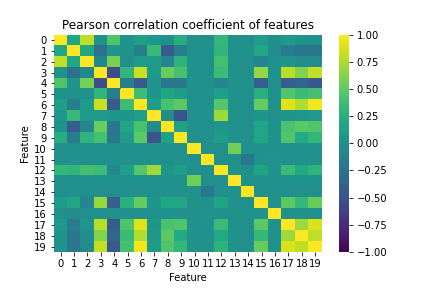
\includegraphics[width=\textwidth]{pearson.png}
%  \end{minipage}
%  \hfill
%  \begin{minipage}{0.235\textwidth}
%    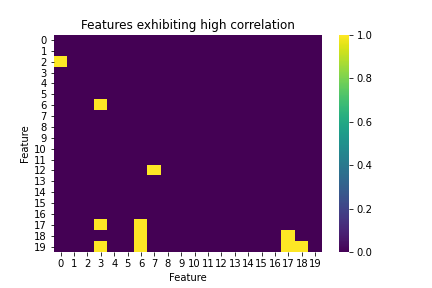
\includegraphics[width=\textwidth]{high_corr_features.png}
%  \end{minipage}
%  \caption{Pearson correlation heatmap of all features (left) and after applying correlation threshold of 0.7 for lower triangular matrix (right)}
%  \label{fig:corr}
%\end{figure}


\begin{figure}
  \centering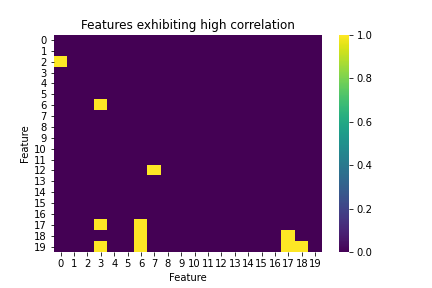
\includegraphics[width=0.8\linewidth]{high_corr_features.png}
  \caption{Pearson correlation heatmap of lower triangular matrix of features after applying correlation threshold of 0.7}
  \label{fig:corr}
\end{figure}

Finally, we apply polynomial expansion to our dataset. Specifically, for each feature $x$, we concatenate columns representing $x^2$, $x^3$, ... , $x^{degree}$ where cross validation is performed for the ideal degree value. The final number of features will be $14 \times degree + 1$.


\section{Models and Methods}
\label{sec:methods}

\subsection{Models}

The six machine learning algorithms are the following:
\begin{enumerate}
  \item Linear regression using gradient descent (GD)
  \item Linear regression using stochastic gradient descent (SGD)
  \item Least squares regression using normal equations
  \item Ridge regression using normal equations
  \item Logistic regression using GD
  \item Regularized logistic regression using GD
\end{enumerate}

\subsection{Hyperparameters}
The hyperparameters selected lie in the following ranges:
\begin{enumerate}
  \item $\gamma \in \{10^{-1}, 10^{-2}, 10^{-3}, 10^{-4}, 10^{-5}, 10^{-6}\}$
  \item $\lambda \in \{10^{-2}, 10^{-3}, 10^{-4}, 10^{-5}\}$
  \item $iterations \in \{1000, 2000, 3000\}$
  \item $degree \in \{5, 7, 9\}$
\end{enumerate}

\subsection{Cross Validation}
To validate the model, a 5-fold cross validation is used on the training set. This technique splits the dataset in five equivalent bins where each bin is selected as the test bin, and the four remaining ones are used to train the model. The resulting hyperparameters and its corresponding accuracy for each method is outlined in Table \ref{tab:hyper}. 

\begin{table}[h!]
  \centering
  \caption{Hyperparameters obtained with 5-fold cross validation}
  \begin{tabular}{|l||c|c|c|c|c|}
      \hline
      \textbf{Model} & \textbf{$\gamma$} & \textbf{$\lambda$} & \textbf{iter.} & \textbf{deg.} & \textbf{acc.}\\ \hline\hline
      Linear regression GD & 0.1 & - & 2000 & - & 70.7\%\\ \hline
      Linear regression SGD & 0.001 & - & 2000 & - & 69.7\%\\ \hline
      Least squares & - & - & - & 9 & 78.1\%\\ \hline
      Ridge regression & - & $2.7\cdot10^{-3}$ & - & 9 & 78.2\%\\ \hline
      Logistic regression & 0.001 & - & 2000 & 1 & 70.3\%\\ \hline
      Reg. logistic regression & 0.001 & $6.3\cdot10^{-4}$ & 2000 & 1 & 70.3\%\\ \hline
  \end{tabular}
  \label{tab:hyper}
\end{table} 

The learning rate ($\gamma$) for the required methods were tuned manually by observing the printed losses during training. The model is interrupted should the loss begin to diverge and thus decreased as a result. A maximum iteration of 2000 is chosen for necessary models as this deemed as an appropriate value for obtaining the minimum loss. Increasing the iterations may achieve more optimal results, but come at a cost of computation which was not explored.

We show cross validation plots for ridge and regularized logistic regression in Figures \ref{fig:ridge} and \ref{fig:logistic}, respectively. We observe that the optimal degree for polynomial expansion is 9 for both least squares and ridge regression. This is expected as the higher degree, the more number of features which can be obtained. It was decided to not apply feature augmentation on logistic and regularized logistic regression for computation reasons. As such, its degree is set to 1.

\begin{figure}
  \centering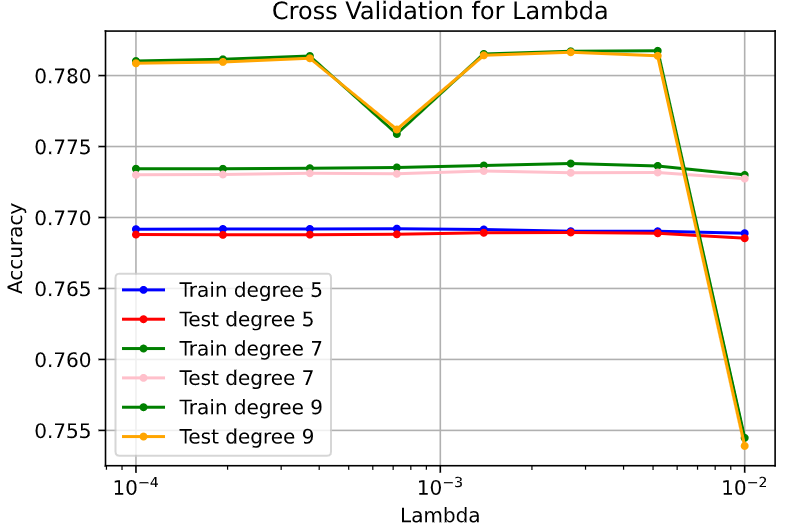
\includegraphics[width=0.8\linewidth]{ridge_reg.png}
  \caption{Cross validation using ridge regression}
  \label{fig:ridge}
\end{figure}

\begin{figure}
  \centering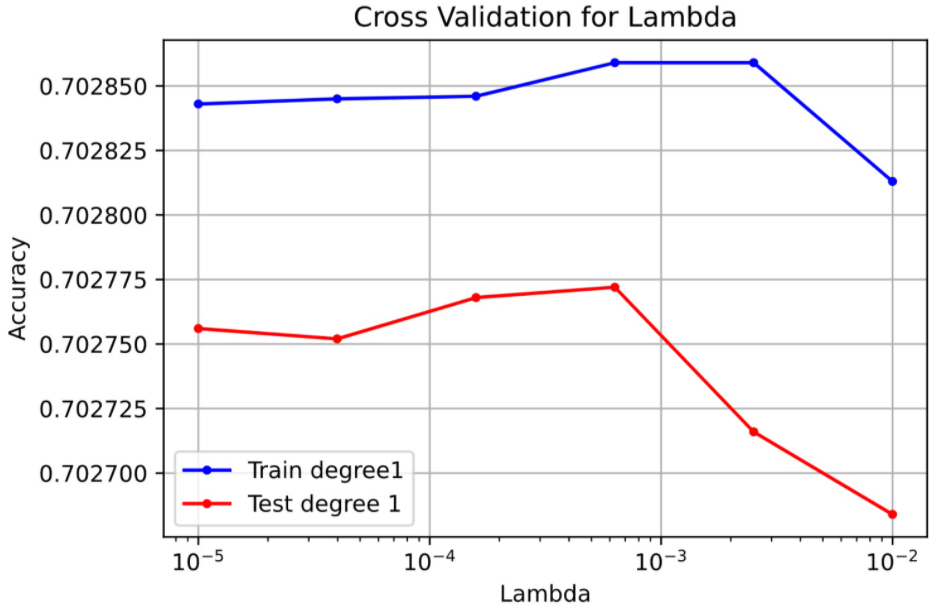
\includegraphics[width=0.8\linewidth]{reg_logist.png}
  \caption{Cross validation using regularized logistic regression}
  \label{fig:logistic}
\end{figure}


\section{Results and Discussion}
\label{sec:results}
From the cross validation results, it can be seen that the favourable algorithm is ridge regression with an accuracy of 78.2\%. The obtained predictions are submitted on \texttt{AIcrowd}, achieving an accuracy of 78\% and an F1 score of 65.8\%. It is also evident in Figure \ref{fig:logistic} that the training accuracy is slightly higher than the testing accuracy, indicating a very minimal overfit model. It is also surprising to see logistic regression as not being the obvious method of choice for binary classification. However, this may be explained for several reasons.

Firstly, logistic regression is an iterative method that requires to solve an optimization problem. As such, a greater number of iterations is beneficial in achieving a higher accuracy. Additionally, feature augmentation was omitted from the methodology which should have improved results. Furthermore, greater reduction of dimensions in the dataset will also attribute to more favourable results. A method such as Principal Component Analysis (PCA) will have simplified the model by identifying ideal features to include in training.

Finally, more sophisticated feature engineering on the dataset will achieve an even higher accuarcy for the proposed models. Such methods may include exploring the \texttt{PRI\_jet\_num} feature as discussed earlier, employing a different feature augmentation such as multiplying pairs of columns, applying a natural logarithm to skewed features and removing features with low variance or poor distributions.

\section{Conclusion}
\label{sec:conclusion}
In the following project, we propose six machine learning algorithms for binary classification of the Higgs boson dataset. The highest performing model was ridge regressions with a maximum accuracy of 78\% on an unlabelled testing set. We employ a series of preprocessing techniques towards the data to improve results and introduce next steps that may even further improve results. 

\begin{thebibliography}{1}
	\bibitem{higgs}
  C. Adam-Bourdarios, G. Cowan, C. Germain, I. Guyon, B. Kegl, and D. Rousseau, “Learning to discover: the Higgs boson machine learning challenge,” 2014.
\end{thebibliography}

\end{document}
